% --------------------------------------------------------------
% This is all preamble stuff that you don't have to worry about.
% Head down to where it says "Start here"
% --------------------------------------------------------------
 
\documentclass[12pt]{article}
 
\usepackage[margin=1in]{geometry} 
\usepackage{amsmath,amsthm,amssymb}
\usepackage[margin=1in]{geometry} 
\usepackage{amsmath,amsthm,amssymb}
\usepackage[english]{babel} 
\usepackage[T1]{fontenc} 
\usepackage[utf8]{inputenc} 
\usepackage{lmodern} 
\usepackage{graphicx}
\graphicspath{ {images/} }
\usepackage{hyperref}
 
\newcommand{\N}{\mathbb{N}}
\newcommand{\Z}{\mathbb{Z}}
 
\newenvironment{theorem}[2][Theorem]{\begin{trivlist}
\item[\hskip \labelsep {\bfseries #1}\hskip \labelsep {\bfseries #2.}]}{\end{trivlist}}
\newenvironment{lemma}[2][Lemma]{\begin{trivlist}
\item[\hskip \labelsep {\bfseries #1}\hskip \labelsep {\bfseries #2.}]}{\end{trivlist}}
\newenvironment{exercise}[2][Exercise]{\begin{trivlist}
\item[\hskip \labelsep {\bfseries #1}\hskip \labelsep {\bfseries #2.}]}{\end{trivlist}}
\newenvironment{problem}[2][Problem]{\begin{trivlist}
\item[\hskip \labelsep {\bfseries #1}\hskip \labelsep {\bfseries #2.}]}{\end{trivlist}}
\newenvironment{question}[2][Question]{\begin{trivlist}
\item[\hskip \labelsep {\bfseries #1}\hskip \labelsep {\bfseries #2.}]}{\end{trivlist}}
\newenvironment{corollary}[2][Corollary]{\begin{trivlist}
\item[\hskip \labelsep {\bfseries #1}\hskip \labelsep {\bfseries #2.}]}{\end{trivlist}}

\newenvironment{solution}{\begin{proof}[Solution]}{\end{proof}}
 
\begin{document}
 
% --------------------------------------------------------------
%                         Start here
% --------------------------------------------------------------
 
\title{Intro to AI and ML}
\author{Anjani Kumar : CS17BTECH11002\\ %replace with your name
Tungadri Mandal : CS17BTECH11043}

\maketitle
\section{Reflection About A Line }
Find the equation of the circle, which is the
mirror image of the circle
% 	Y = 1000 - \frac{600}{4} \times (X-2)
\begin{equation}
    \boldsymbol{x^Tx} - (2\hspace{5mm} 0)\boldsymbol{x} = 0
\end{equation}
in the line 
\begin{equation}
    (1\hspace{5mm} 1)\boldsymbol{x} = 3
\end{equation}
% \
% \[\left\{ \begin{array}{rcl}
% f_{1}=(cos(t),tan(t))
% \\
% f_{2}=(tan(t),sin(t)) 
% & 
% \end{array}
% \right. \]


% An image of the given circle, line and it's mirror image attached
\begin{figure}[h]
\centering
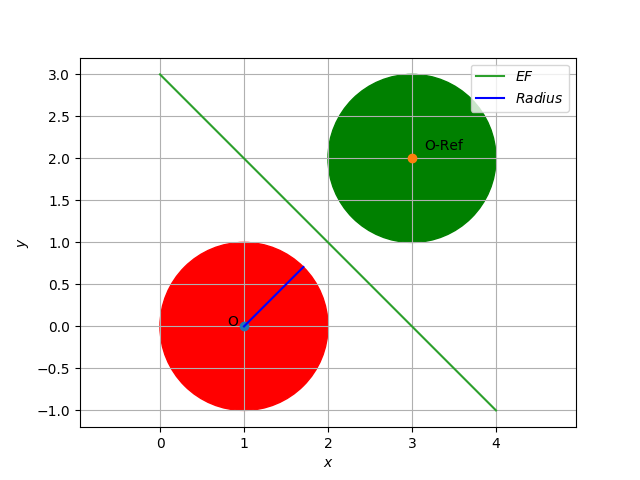
\includegraphics[scale=0.65]{figs/circles.png}
\caption{Reflection of circle about a line}
\label{etiqueta}
\end{figure}

\begin{solution}
Let $\boldsymbol{c}$ be the center and r be the radius of the circle respectively.
\begin{equation}
    \Vert\left(\boldsymbol{x - c}) \right\Vert^2 = r^2
\end{equation}
\begin{equation}
    \Rightarrow \boldsymbol{(x-c)^T(x-c)} = r^2
\end{equation}
\begin{equation}
    \Rightarrow \boldsymbol{x^Tx - 2c^Tx} = r^2 - \boldsymbol{c^Tc}
\end{equation}
Comparing with eqn(1),
\begin{align}
    \boldsymbol{c} &= \begin{bmatrix}
           1 \\
           0 \\
         \end{bmatrix}
\end{align}
\begin{equation}
    r^2 - \boldsymbol{c^Tc} = 0 \Rightarrow r = 1
\end{equation}  
\end{solution}

We have the equation of line as
\begin{equation}
    (1\hspace{5mm} 1)\boldsymbol{x} = 3
\end{equation}
this can be written in the form
\begin{equation}
    \boldsymbol{Nx = } C
\end{equation}
where N is the normal to the line and C is a constant.\\
Comparing with eqn(8),\\
\begin{align}
    \boldsymbol{N} &= \begin{bmatrix}
           1 \\
           1 \\
         \end{bmatrix}
\end{align}

Intersection of line (passing through center $\boldsymbol{c}$ and $\boldsymbol{c + 0.1N}$) with the given line gives the foot of perpendicular on the given line from $\boldsymbol{c}$.\\
Let $\boldsymbol{f}$ and $\boldsymbol{c'}$ be the foot of perpendicular and image of center respectively.\\
Then we have 
\begin{equation}
    \frac{\boldsymbol{c+c'}}{2} = \boldsymbol{f}
\end{equation}
\begin{equation}
    \Rightarrow \boldsymbol{c' = 2f + c}
\end{equation}
Since the radius remains same after reflection, we have equation of reflected circle as 
\begin{equation}
    \boldsymbol{x^Tx - 2c'^Tx} = r^2 - \boldsymbol{c'^Tc'}
\end{equation}
\section{ Walkthrough of the code }

\textbf{function norm\_vec(AB)}\hfill //returns the normal vector of line AB.\\
\textbf{function mid\_pt(B,C)}\hfill //calculates the mid point of two given points.\\
\textbf{function line\_intersect\_normal\_form(N,P)}\hfill //creates a line from normal form.\\
\textbf{function line\_intersect\_normal\_form(N,P)}\hfill //returns reflection of a point about a line.\\
\\
\textbf{MAIN SECTION}\\
// centre of the circle \\
\textbf{cen=np.matmul(cenM,A.T)} \\
\\
// constant term for the circle \\
\textbf{D=0} \\
\\
// Reflected centre \\
\textbf{refCen=reflection\_normal\_form(B,C,cen)} \\
\\
// Radius of the circle \\
\textbf{radius=(cen[0]**2+cen[1]**2-D)**0.5} \\
\\
// Foot of perpendicular of the center to the line \\
\textbf{E=(cen+refCen)/2} \\


% --------------------------------------------------------------
%     You don't have to mess with anything below this line.
% --------------------------------------------------------------
 
\end{document}